\documentclass{uebblatt}

\begin{document}

\maketitle{3}{\emph{Jedes Konzept ist eine Kan-Erweiterung.}}

\begin{aufgabe}{Kan-Erweiterungen von darstellbaren Koprägarben}
Sei~$K : \M \to \C$ ein Funktor. Zeige:
$\operatorname{Lan}_K \Hom_\M(X, \smallplaceholder) =
  \Hom_\C(K(X), \smallplaceholder)$.
\end{aufgabe}

\begin{aufgabe}{Die Limesformel für punktweise Kan-Erweiterungen}
Sei~$K : \M \to \C$ ein Funktor. Sei~$T : \M \to \A$ ein Funktor derart, dass
für alle Objekte~$c \in \C$ der Limes~$R(c) \defeq \lim_{f:K(m) \to c} T(m)$
existiert.
% Die Indexkategorie des Limes sieht also wie folgt aus:
% Objekte der Indexkategorie sind Morphismen K(m) --> c, wobei m aus M beliebig
% sein kann.
% Morphismen zwischen K(m) --> c und K(m') --> c sind Morphismen g : m --> m'
% derart, dass das Dreieck mit den Kanten K(g), K(m') --> c und K(m) --> c
% kommutiert.
\begin{enumerate}
\item Erkläre, wie man diese Setzung zu einem Funktor~$R : \C \to \A$ ausdehnen
kann.
\item Beweise, dass~$R$ eine Rechts-Kan-Erweiterung von~$T$ längs~$K$ wird.
\end{enumerate}
\end{aufgabe}

\begin{aufgabe}{Kan-Erweiterungen längs volltreuer Funktoren}
Sei~$K : \M \to \C$ ein volltreuer Funktor. Sei~$T : \M \to \A$ ein Funktor
derart, dass die punktweise Links-Kan-Erweiterung~$\mathrm{Lan}_K(T)$
existiert. Zeige: Die kanonische natürliche Transformation~$T \Rightarrow
\mathrm{Lan}_K(T) \circ K$ ist ein Isomorphismus.

{\tiny\emph{Tipp:} Die Kolimesformel für~$\mathrm{Lan}_K(T)$ lässt sich stark
vereinfachen.\par}
\end{aufgabe}

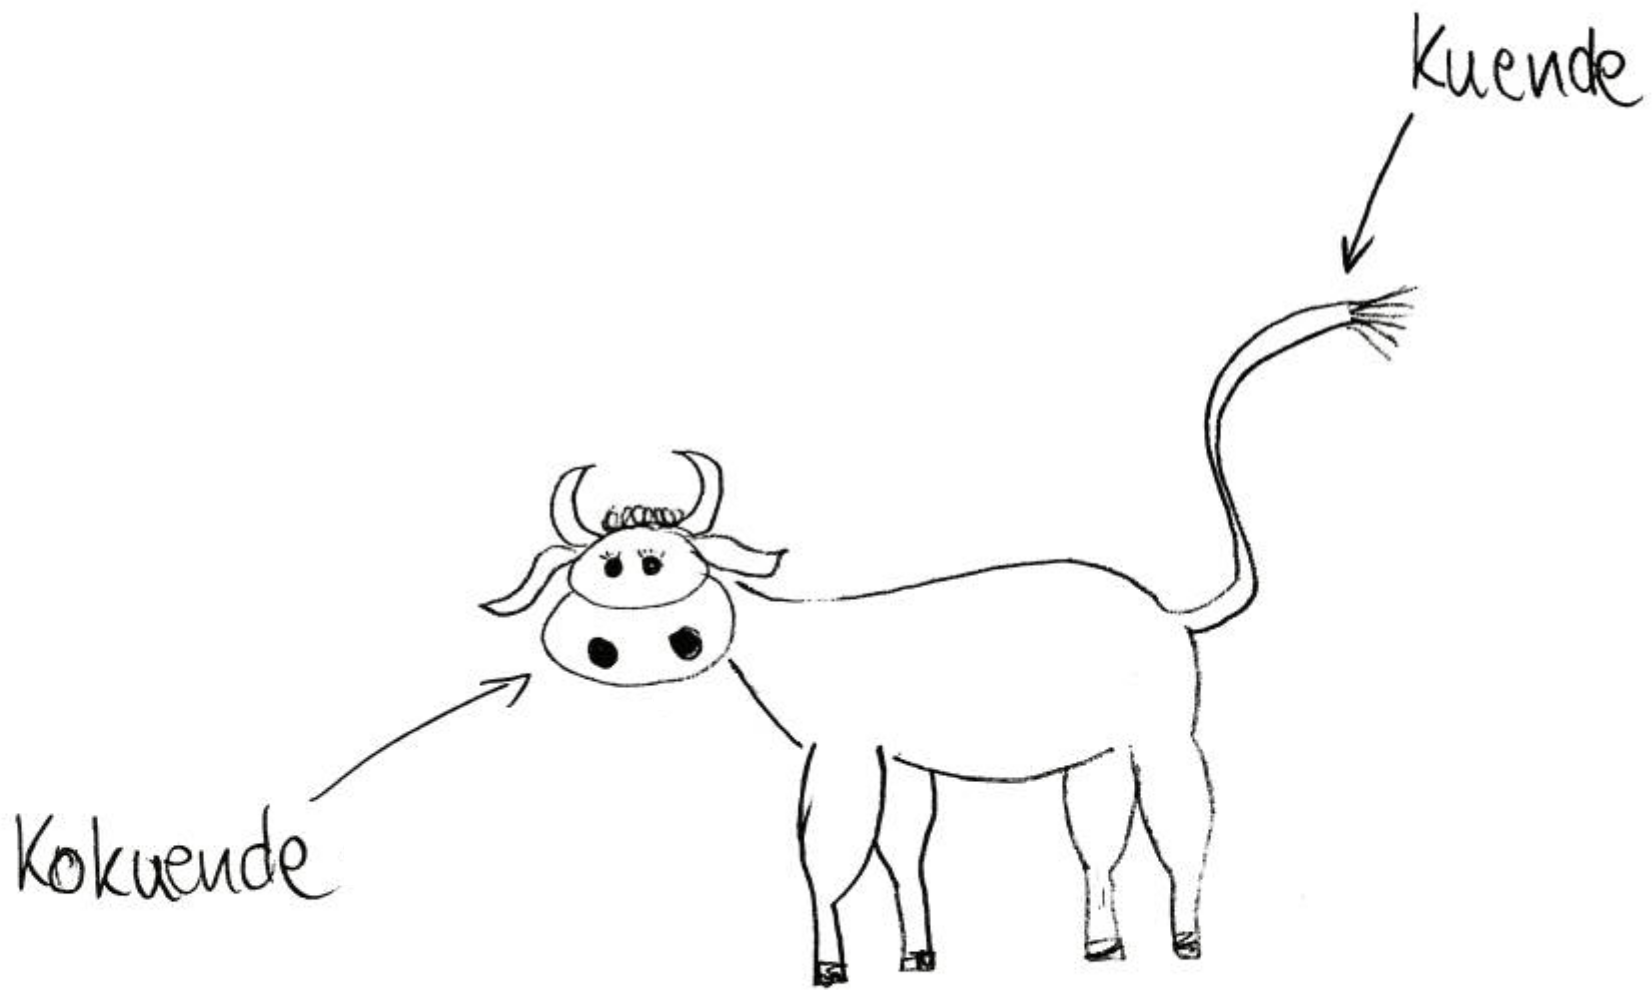
\includegraphics{images/kuende}

\end{document}

\begin{aufgabe}{Vertauschbarkeit von filtrierten Kolimiten mit endlichen Limiten}
Sei~$F : \C \times \D \to \Set$ ein Funktor.
\begin{enumerate}
\item Konstruiere einen kanonischen Morphismus~$\lambda : \colim\limits_{c \in \C}
\lim\limits_{d \in D} F(c,d) \to \lim\limits_{d \in \D} \colim\limits_{c \in \C} F(c,d)$.
\item Sei~$\C$ sogar eine filtrierte Kategorie. Zeige, dass dann~$\lambda$ ein Isomorphismus ist.
\end{enumerate}
\end{aufgabe}
